\section{Why change?} % (fold)
\label{sec:why_change_}

\begin{frame}{Last update?}
\begin{Parallel}[v]{5cm}{5cm}
    \ParallelLText%
    {

        {\ttfamily Clang}  13 July of 2015
    }
    \ParallelRText%
    {
        {\ttfamily DoxyParse} 18 January of 2013
	}
\end{Parallel}
\end{frame}

\begin{frame}{What Doxygen is?}
   \begin{itemize} 
        \item Doxygen is a software for documentation
        \item Doxygen is way ahead of doxyparse
        \item DoxyParse has a few number of maintainers
    \end{itemize} 
\end{frame}

\begin{frame}{What Clang is?}
   \begin{itemize} 
        \item Clang is a huge compiler  
        \item Clang is constantly updated
        \item Clang has perl bindings
        \item Clang is suported by important companies
    \end{itemize}
\end{frame}

% section why_change (end)

\section{How it works} % (fold)
\label{sec:how_it_works}

\begin{frame}{Clang $\times$ Doxyparse}
% how_it_works.png
% \begin{figure}[htbp]
    \centering
        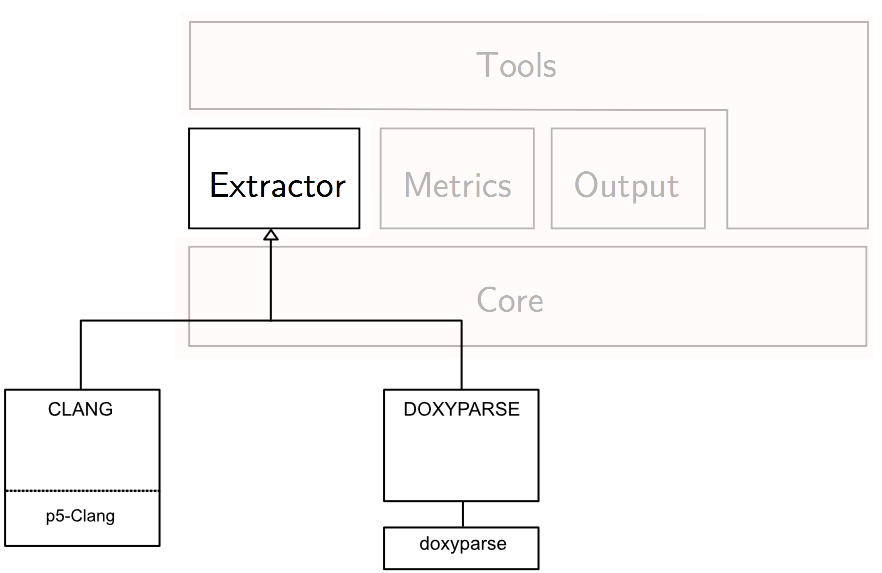
\includegraphics[width=0.9\textwidth]{conteudo/how_it_works.png}
    % \caption{}
    % \label{fig:tipografia}
% \end{figure}
\end{frame}

\section{P5-Clang} % (fold)
\label{sec:p5_clang}

\subsection*{Contributions}
\begin{frame}{Cursors}
    \begin{itemize} 
        \item Final line of functios and classes  
        \item Access Specifier
        \item Virtual or pure Virtual method
        \item Number of arguments
        \item Unified symbol resolution (USR)
        \item Member refers to system header
        \item Caller of a statement 
    \end{itemize}
\end{frame}

\begin{frame}{Plus}

\begin{itemize}
    \item Test refactoring
    \item LLVM support updated from 3.3 (17 Jun 2013) to 3.5 (20 Jan 2015)
\end{itemize}
    
\end{frame}

\section{To do} % (fold)
\label{sec:analizo}

\begin{frame}{What still missing?}
    \begin{itemize} 
        \item Clang as default extractor
        \item Call between functions   
        \item Functional tests
        \item Fix tests
    \end{itemize}
\end{frame}
